\documentclass{article}
\usepackage[utf8]{inputenc}
\usepackage[english]{babel}
\usepackage{url}
\usepackage{graphicx}
\usepackage{geometry}
\usepackage{amsmath}
\usepackage{subcaption}
\usepackage{xcolor}
\usepackage{amsmath,accents}
\usepackage{physics}
\usepackage{setspace}
\usepackage{caption}
\usepackage{float}
\usepackage[makeroom]{cancel}
\usepackage{multicol}
\newcommand{\myvect}[1]{\accentset{\rightharpoonup}{#1}}
\usepackage[round]{natbib}
\bibliographystyle{unsrtnat}
\usepackage{tikz}
\usetikzlibrary{calc}
\usetikzlibrary{angles,quotes} % for pic
\usetikzlibrary{bending} % for arrow head angle
\tikzset{>=latex} % for LaTeX arrow head

\colorlet{xcol}{blue!70!black}
\colorlet{vcol}{green!60!black}
\colorlet{pcol}{red!60!black}
\colorlet{Lcol}{green!50!black}
\colorlet{myred}{red!65!black}
\colorlet{mypurple}{blue!60!red!80}
\colorlet{acol}{red!50!blue!80!black!80}
\tikzstyle{rvec}=[->,xcol,very thick,line cap=round]
\tikzstyle{vvec}=[->,vcol,very thick,line cap=round]
\tikzstyle{pvec}=[->,pcol,very thick,line cap=round]
\tikzstyle{Lvec}=[->,Lcol,very thick,line cap=round]
\tikzstyle{mass}=[line width=0.6,red!30!black,draw=red!30!black,
                  top color=red!40!black!30,bottom color=red!40!black!10,shading angle=30]
\doublespacing
\setlength\parindent{24pt}

\begin{document}

\begin{titlepage}
    \begin{center}
    \vspace*{1cm}
        
        \textbf{Studying the precession of a bicycle wheel}
        
        \vspace{0.5cm}
        What gyroscopic influences does the front wheel of a bicycle have when torque is applied to the system?\\
        \vspace{1.5cm}
        Word Count: 3839
        \vfill
        
        Physics Extended Essay presented\\
        for the International Baccalaureate Degree
        
        \vspace{0.8cm}
        
        candidate number
        
    \end{center}
\end{titlepage}

\tableofcontents
\pagebreak
\section{Introduction}

In this extended essay, we will look into the gyroscopic effect the front wheel has on a bike while experiencing an induced torque. The experiment looks to find the relation between the speed of the spinning wheel and the amount precession experienced by the front wheel.

To understand the mechanics behind the precession of said wheel, we will be looking at precession, and explaining it in an intuitive and in-depth fashion. This is especially interesting and useful since precession is the main mechanism in spinning tops, boat gyroscopes (devices used to stabilize boats), and many other common day occurrences. Although I have not seen precession as part of my course, I found it to be an area of interest due to its inherent complexity but also great relevance.

As a mountain biker myself, this topic comes into full contact with my interests, as it's useful not only to know what are the forces involved with riding a bike but more importantly, a better grasp of the mechanics that go behind riding a bicycle. A better understanding of what is happening with a bicycle might shed some light on a better understanding of the physics behind riding one (\cite{hubbard2011human,kooijman2006experimental,meijaard2007linearized}).

In essence, this extended essay stands as a testament to the ceaseless curiosity of scientific inquiry. The physical properties of gyroscopes do not cease to amaze, and a better understanding of their physics may bring clarity, and in collaboration, knowledge.

\pagebreak
\subsection{Introduction to circular motion}
Circular motion is a part of classical physics, whereas the study of masses spinning around an axis is performed. This area of physics involves many different phenomena as angular velocity, angular momentum, and many others (\cite{precession,angularvelocity,momentofinertia}). These will be useful to better understand precession.

To simplify and generalize our equations, we will assume the bodies here to be rigid. This means we can assume force to be equal to the derivative of mass times velocity against time (or force to be equal to the derivative of momentum taking that mass doesn't change over time). Therefore, for our purposes, we can take Newton's second law of motion as true(\cite{angularvelocity}).

\begin{equation}
    \myvect{\text{\textbf{F}}}=\frac{d}{dt}(\text{m}\myvect{\text{\textbf{v}}})=\frac{d\myvect{\text{\textbf{p}}}}{dt}
\end{equation}

Through this preconception, we can set some bases. First and foremost, we will consider a change of angle through an axle $\Delta\Theta$ (or the difference of two angles). From that, we can assume a disk making a full rotation has a change of angle of 2$\pi$ or 360$^{\circ}$. Through this, we can define angular velocity as the change in angular velocity through time, or $\frac{\Delta\Theta}{\Delta t}$. Angular velocity is conventionally notated as $\myvect{\omega}$. Since angular velocity does represent a rotation in a specific direction, it is vectorial. It is also important to note the relation between angular velocity and frequency, where $\myvect{\omega}=2\pi f$. Following this logic, the change of angular velocity through time is $\frac{\Delta\myvect{\omega}}{\Delta t}$ and is usually referred to as $\alpha$. Following are the combined equations previously mentioned, displayed more suitably.

\begin{equation*}
\begin{aligned}
    \Delta\Theta =& \Theta_1 - \Theta_2\\
    \omega =& \frac{\Delta\Theta}{\Delta t}\\
    \myvect{\alpha} =& \frac{\Delta\myvect{\omega}}{\Delta t}\\
\end{aligned}
\end{equation*}

These are, in a basic way, the kinematics of circular motion (\cite{angularvelocity}). Looking now at the dynamics of circular motion, we have a few things to unpack. Since we are not moving a mass around, but spinning it, instead of using mass, we use I, representing an object's resistance to its rotation. The calculation process of I is quite complex (and usually given), however in some cases (including in our experiment) we can calculate it through more involving processes. It is also known as the moment of inertia of an object. In circular motion, force also cannot be used, since it usually is useful in linear motion, but instead, torque is used. Torque is equal to the angular acceleration times I. Simply put, it is a twisting force. It can also be described as the cross-product of a force and the axis of rotation.

An important measure for this article is the angular momentum. Angular momentum is represented by $\myvect{\textbf{L}}$, and is equal to to the sum of the cross products of momentum and axis of rotation between all points of mass in the object (\cite{momentofinertia,listofmomentofinertia}). Alternatively, it is also equal to the multiplication between I and angular velocity. Angular momentum is crucial in the understanding of precession and therefore can be seen represented in figure~\ref{fig:Diagram of angular momentum}.

\begin{figure}[H]
\centering
    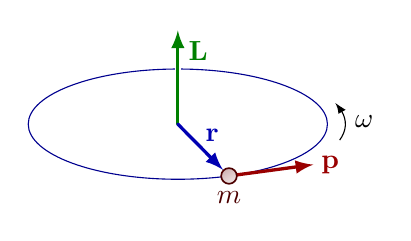
\begin{tikzpicture}
    \def\R{1.9}   % circle radius
    \def\Ry{0.7}  % circle radius
    \def\r{1.4}   % mass radius (inner sep)
    \def\ang{-70} % mass angular position
    \coordinate (O) at (0,0);
    \coordinate (L) at (0,1.7*\Ry);
    \coordinate (R) at (\ang:{\R} and \Ry);
    \draw[xcol!80!black] (O) ellipse({\R} and \Ry);
    \draw[pvec] (R) --++ (\ang+90:{0.6*\R} and 0.6*\Ry) node[right=-1] {$\vb{p}$};
    \node[mass,circle,inner sep=2] (R') at (R) {};
    \node[red!30!black,below=2] at (R') {$m$};
    \draw[white,line width=2] (O) -- (L);
    \draw[Lvec] (O) -- (L) node[below right=0] {$\vb{L}$};
    \draw[rvec] (O) -- (R') node[midway,above right=-2] {$\vb{r}$};
    \draw[-{>[bend]}] (-15:{1.12*\R} and {1.12*\Ry}) arc(-15:20:{1.12*\R} and {1.12*\Ry})
    node[pos=0.5,right] {$\omega$};
    \end{tikzpicture}
\caption{Diagram of angular momentum} 
\label{fig:Diagram of angular momentum}
\end{figure}

This figure can give us a better grasp of understanding the relationship the angular momentum has with momentum and points of mass. This concludes the useful part of dynamics we will be using throughout the paper. Following are the equations for dynamics.

\begin{equation*}
\begin{aligned}
    \myvect{\tau} =& \myvect{\text{F}}\myvect{\text{r}}\,\sin{\Theta}\\
    \myvect{\tau} =& \myvect{\alpha}\,\text{I}\\
    \myvect{\text{L}} =& \sum\myvect{\textbf{r}}\cross\myvect{\textbf{p}}\\
    \myvect{\text{L}} =& \myvect{\omega}\,\text{I}\\
\end{aligned}
\end{equation*}

\pagebreak
\subsection{Introduction to precession}
Precession is by definition the act of an axis spinning around a second axis non-parallel to the first one. This physical phenomenon is commonly seen in day-to-day life, with its most widespread example being the spinning of a top. For our interests, torque-induced precession will be the extent of our research. Torque-induced precession happens when a gyroscope (a spinning wheel or disc that can rotate quickly around an axis that can change direction) feels an external torque. This leads to a change in the angular momentum (\cite{precession,precessioncomplex}). The equation for torque-induced precession is is: $\myvect{\tau} = \frac{d\myvect{\text{L}}}{d\text{t}}$. To better visualize with an example, we can see figure~\ref{fig:Diagram of a spinning top experiencing torque-induced precession}, where a diagram of a spinning top experiencing precession can be viewed.

\begin{figure}[!ht]
\centering
\includegraphics[width=0.5\textwidth]{img/precession.jpg}
\caption{Diagram of a spinning top experiencing torque-induced precession (\cite{precessiondiagram})}
\label{fig:Diagram of a spinning top experiencing torque-induced precession}
\end{figure}

It can be observed in the image the aforementioned change in angular momentum. The diagram only shows us the change in angular momentum and the angular velocity of precession. What it fails to show us is the torque of the precession. A description of the exerted torque of the torque-induced precession can be done through calculations as seen in other scientific papers (\cite{lagutin2021spinning}).

\begin{equation*}
\begin{aligned}
    \myvect{\tau}_{exerted\,by\,precession} =& \frac{d\myvect{\text{L}}}{d\text{t}}\\
    \myvect{\tau}_{exerted\,by\,precession} =& \frac{d(\text{I}_{wheel}\,\omega _{wheel\,precession})}{d\text{t}}\\
    \myvect{\tau}_{exerted\,by\,precession} =& \frac{d(\text{I}_{wheel})}{d\text{t}}\omega_{wheel\,precession} + \text{I}\,\alpha_{wheel\,precession}\\
\end{aligned}
\end{equation*}

This however is not yet useful, as it is needed that we equate our system with those preconceptions in mind. Firstly, to better understand out setup, a diagram is in order as to show the variables that will be put into place. The setup itself will be further explain in the method section.

\begin{figure}[H]
\centering
    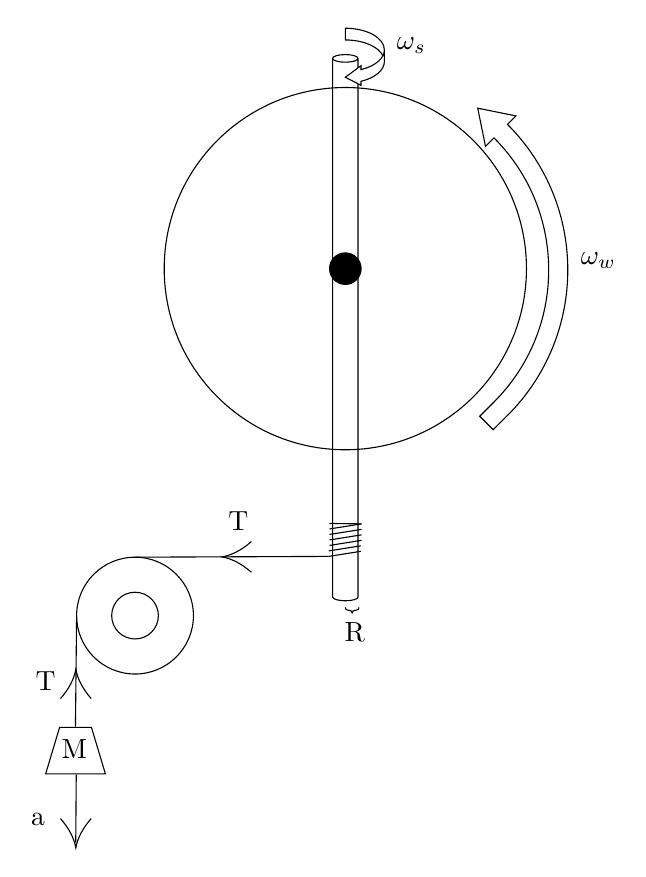
\begin{tikzpicture}[x=0.85pt,y=0.85pt,yscale=-1,xscale=1]
    %uncomment if require: \path (0,422); %set diagram left start at 0, and has height of 422
    
    %Shape: Can [id:dp7833299946361889] 
    \draw   (335.8,39.62) -- (335.8,268.58) .. controls (335.8,269.47) and (333.38,270.2) .. (330.4,270.2) .. controls (327.42,270.2) and (325,269.47) .. (325,268.58) -- (325,39.62) .. controls (325,38.73) and (327.42,38) .. (330.4,38) .. controls (333.38,38) and (335.8,38.73) .. (335.8,39.62) .. controls (335.8,40.51) and (333.38,41.24) .. (330.4,41.24) .. controls (327.42,41.24) and (325,40.51) .. (325,39.62) ;
    %Shape: Circle [id:dp09376020346777403] 
    \draw   (253.4,129) .. controls (253.4,86.47) and (287.87,52) .. (330.4,52) .. controls (372.93,52) and (407.4,86.47) .. (407.4,129) .. controls (407.4,171.53) and (372.93,206) .. (330.4,206) .. controls (287.87,206) and (253.4,171.53) .. (253.4,129) -- cycle ;
    %Straight Lines [id:da045558907326921916] 
    \draw    (323.67,237.33) -- (337.33,237.5) ;
    %Straight Lines [id:da4340730712106843] 
    \draw    (323.67,239.67) -- (337.33,237.5) ;
    %Straight Lines [id:da8272486950812334] 
    \draw    (323.67,242) -- (337.33,239.83) ;
    %Straight Lines [id:da3182515925644319] 
    \draw    (323.67,244.33) -- (337.33,242.17) ;
    %Straight Lines [id:da16165035762131374] 
    \draw    (323.67,246.67) -- (337.33,244.5) ;
    %Straight Lines [id:da8950622367779497] 
    \draw    (323.33,249) -- (337,246.83) ;
    %Straight Lines [id:da48665687178927153] 
    \draw    (323.33,251.33) -- (337,249.17) ;
    %Straight Lines [id:da01589096261852674] 
    \draw    (241,251.67) -- (323.33,251.33) ;
    %Shape: Donut [id:dp2965336832053179] 
    \draw   (231.07,276.5) .. controls (231.07,271.01) and (235.51,266.57) .. (241,266.57) .. controls (246.49,266.57) and (250.93,271.01) .. (250.93,276.5) .. controls (250.93,281.99) and (246.49,286.43) .. (241,286.43) .. controls (235.51,286.43) and (231.07,281.99) .. (231.07,276.5)(216.17,276.5) .. controls (216.17,262.78) and (227.28,251.67) .. (241,251.67) .. controls (254.72,251.67) and (265.83,262.78) .. (265.83,276.5) .. controls (265.83,290.22) and (254.72,301.33) .. (241,301.33) .. controls (227.28,301.33) and (216.17,290.22) .. (216.17,276.5) ;
    %Straight Lines [id:da7185578103952567] 
    \draw    (215.67,323.67) -- (216.17,276.5) ;
    %Shape: Trapezoid [id:dp05405151896010563] 
    \draw   (203,343.8) -- (208.94,324) -- (222.47,324) -- (228.41,343.8) -- cycle ;
    %Shape: Brace [id:dp46700395171891906] 
    \draw   (330.4,273) .. controls (330.4,273.79) and (330.8,274.19) .. (331.59,274.19) -- (331.59,274.19) .. controls (332.73,274.19) and (333.3,274.59) .. (333.3,275.39) .. controls (333.3,274.59) and (333.87,274.19) .. (335.01,274.19)(334.49,274.19) -- (335.01,274.19) .. controls (335.8,274.19) and (336.2,273.79) .. (336.2,273) ;
    \draw   (209.3,311.8) .. controls (212.93,307.63) and (215.11,303.47) .. (215.84,299.3) .. controls (216.57,303.47) and (218.75,307.63) .. (222.38,311.8) ;
    \draw   (290.49,258.09) .. controls (286.32,254.46) and (282.16,252.28) .. (277.99,251.55) .. controls (282.16,250.82) and (286.32,248.64) .. (290.49,245.01) ;
    %Shape: Circle [id:dp627318229619773] 
    \draw  [fill={rgb, 255:red, 0; green, 0; blue, 0 }  ,fill opacity=1 ] (323.7,129) .. controls (323.7,125.3) and (326.7,122.3) .. (330.4,122.3) .. controls (334.1,122.3) and (337.1,125.3) .. (337.1,129) .. controls (337.1,132.7) and (334.1,135.7) .. (330.4,135.7) .. controls (326.7,135.7) and (323.7,132.7) .. (323.7,129) -- cycle ;
    %Curve Right Arrow [id:dp13230993256922918] 
    \draw  [fill={rgb, 255:red, 255; green, 255; blue, 255 }  ,fill opacity=1 ] (347,40.96) .. controls (347,35.89) and (339.57,31.78) .. (330.4,31.78) -- (330.4,26.8) .. controls (339.57,26.8) and (347,30.91) .. (347,35.98) ;\draw  [fill={rgb, 255:red, 255; green, 255; blue, 255 }  ,fill opacity=1 ] (347,35.98) .. controls (347,39.74) and (342.9,42.98) .. (337.04,44.4) -- (337.04,42.74) -- (330.4,47.65) -- (337.04,51.04) -- (337.04,49.38) .. controls (342.9,47.96) and (347,44.72) .. (347,40.96)(347,35.98) -- (347,40.96) ;
    %Bend Arrow [id:dp049925041218739086] 
    \draw   (393.27,197.48) -- (399.34,191.41) .. controls (433.51,157.25) and (433.51,101.86) .. (399.34,67.7) -- (399.34,67.7) -- (402.97,64.08) -- (386.69,60.79) -- (389.99,77.06) -- (393.61,73.44) -- (393.61,73.44) .. controls (424.6,104.43) and (424.6,154.68) .. (393.61,185.68) -- (387.54,191.75) -- cycle ;
    %Straight Lines [id:da20762891108195258] 
    \draw    (347,35.98) -- (347,40.96) ;
    %Straight Lines [id:da2816955997800902] 
    \draw    (216.01,344.1) -- (215.8,373) ;
    \draw   (222.37,362.77) .. controls (218.74,366.93) and (216.56,371.1) .. (215.84,375.27) .. controls (215.11,371.1) and (212.93,366.93) .. (209.3,362.77) ;
    
    % Text Node
    \draw (208.7,328) node [anchor=north west][inner sep=0.75pt]   [align=left] {M};
    % Text Node
    \draw (329,278.4) node [anchor=north west][inner sep=0.75pt]   [align=left] {R};
    % Text Node
    \draw (197.6,299.2) node [anchor=north west][inner sep=0.75pt]   [align=left] {T};
    % Text Node
    \draw (279.6,231.2) node [anchor=north west][inner sep=0.75pt]   [align=left] {T};
    % Text Node
    \draw (351.2,29.6) node [anchor=north west][inner sep=0.75pt]   [align=left] {$\omega_{s}$};
    % Text Node
    \draw (429.47,121) node [anchor=north west][inner sep=0.75pt]   [align=left] {$\omega_{w}$};
    % Text Node
    \draw (195.6,359.6) node [anchor=north west][inner sep=0.75pt]   [align=left] {a};
    
    
    \end{tikzpicture}
\caption{Diagram of method of second part of the experiment} 
\label{fDiagram of method of second part of the experiment}
\end{figure}

Through the diagram, it is possible relate the torque to the tension of the string, giving the following equations:

\begin{equation*}
\begin{aligned}
    \text{T}=&\,\text{G}(\text{g}-\text{a})\\
    \myvect{\tau}=&\,\frac{d\myvect{\text{L}}}{d\text{t}}\\
    \myvect{\tau}=&\,\text{G}(\text{g}-\myvect{\text{a}})\cdot\text{R}\\
\end{aligned}
\end{equation*}

The next step is the to proceed with the derivation of the angular momentum. Keep in mind, that although is seems as there were only one moment on inertia, in reality the position vector in the moment of inertia of the system gives two different 'groups' that represent the two axis in which the wheel is rotating. This gives the following equations:

\begin{equation*}
\begin{aligned}
    \frac{d\myvect{\text{L}}}{d\text{t}}=&\frac{d\text{I}_w\cdot\omega_{w}}{d\text{t}}+\frac{d\text{I}_s\cdot \omega_{s}}{d\text{t}}\cdot \omega_{s}\\
    \frac{d\myvect{\text{L}}}{d\text{t}}=&\,\cancelto{o}{\frac{d\text{I}_w}{d\text{t}}\cdot \omega_{w}} + \frac{d\myvect{\omega}_{w}}{d\text{t}}\cdot\text{I}_w + \cancelto{o}{\frac{d\text{I}_s}{d\text{t}}\cdot \omega_{s}} + \frac{d\myvect{\omega}_{s}}{d\text{t}}\cdot\text{I}_s\\
    \frac{d\myvect{\omega}_{w}}{d\text{t}}=&\cancelto{o}{\frac{d{\omega}_{w}}{d\text{t}}}\cdot\myvect{\text{u}} + \frac{d\myvect{\text{u}}}{d\text{t}}\cdot\omega_{w}= {\omega}_{w} \cdot \myvect{\omega}_{s}\\
    \frac{d\myvect{\text{L}}}{d\text{t}}=& {\omega}_{w} \cdot \myvect{\omega}_{s}\cdot\text{I}_w+\frac{d\myvect{\omega}_{s}}{d\text{t}}\cdot\text{I}_s\\
\end{aligned}
\end{equation*}

The derivation of the unit vector $\myvect{\text{u}}$ can be assumed to be equal to $\omega_{s}$, since through logic, the change in direction is the same as the spin of the vertical axis (\cite{IBphysics}). This may be further understood by looking at the diagram in figure~\ref{fDiagram of method of second part of the experiment}. The equation used to get there is the following:

\begin{equation*}
\begin{aligned}
    \frac{d\myvect{\text{u}}}{d\text{t}}=& \lim_{\Delta t\to 0} \frac{\Delta\myvect{\text{u}}}{\Delta\text{t}}=\lim_{\Delta t\to 0} \frac{\Delta\Theta}{\Delta\text{t}}=\omega_{s}\\
\end{aligned}
\end{equation*}

Now, equations can be equated, where the torque and derivative of the moment of inertia are equal to each other. The result aimed for is a functions of v($\omega_w$) with some constants and the moment of inertia $\text{I}_s$, which can then be calculated.

\begin{equation*}
\begin{aligned}
    \text{M}(\text{g}-\text{a}) \cdot \text{R} =& \,\omega_{s}\cdot\omega_{w}\cdot\text{I}_w+\frac{d\myvect{\omega}_{s}}{d\text{t}}\cdot\text{I}_s\\
    \text{M}(\text{g}-\text{a}) \cdot \text{R} =& \,\frac{\text{v}}{\text{R}}\cdot\omega_{w}\cdot\text{I}_w+\frac{d\myvect{\omega}_{s}}{d\text{t}}\cdot\text{I}_s\\
\end{aligned}
\end{equation*}

Rewriting $\frac{d\myvect{\omega}{s}}{d\text{t}}$ as the angular acceleration of the axis (or $\alpha_s$), it can further be equated to $\frac{a}{R}$ due to the setup, where the equation $\alpha = \frac{a{\text{linear}}}{\text{R}}$ holds true since there is no slip in the string. For the same reason, $\omega_{s}$ is assumed to be equal to $\frac{\text{v}}{\text{R}}$

\begin{equation*}
\begin{aligned}
    \text{M}(\text{g}-\text{a}) \cdot \text{R} =& \,\frac{\text{v}}{\text{R}}\cdot\omega_{w}\cdot\text{I}+\frac{\text{a}}{\text{R}}\cdot\text{I}_s\\
    \text{M}\,\text{R}^2\text{g} - \,\text{v}\cdot\omega_{w}\cdot\text{I}_w =& \text{M}\text{g}\,\text{R}^2\text{a}+\text{I}_s\cdot\text{a}\\
    \frac{\text{M}\,\text{R}^2\text{g} - \,\text{v}\cdot\omega_{w}\cdot\text{I}_w}{\text{M}\text{g}\,\text{R}^2+\text{I}_s}=& \text{a}
\end{aligned}
\end{equation*}

Here a problem arises. Further progress with our current tools is not possible, but it can indeed be continued. The equation involves acceleration and speed, or in other words, $x$ and its derivative. This is known as a first degree differential equation. In order to obtain the desired equation, the first degree differential equation is solved as normal (\cite{IBmath}).

\begin{equation*}
\begin{aligned}
    \frac{d\text{v(t)}}{d\text{t}}=&\frac{\text{M}\,\text{R}^2\text{g} - \,\text{v}\cdot\omega_{w}\cdot\text{I}_w}{\text{M}\,\text{R}^2+\text{I}_s}\\
    \frac{d\text{v(t)}}{d\text{t}}=&\frac{\text{M}\,\text{R}^2\text{g}}{\text{M}\,\text{R}^2+\text{I}_s}-\frac{\omega_{w}\cdot\text{I}_w}{\text{M}\,\text{R}^2+\text{I}_s}\cdot\text{v}\\
    \text{v(t)}=&\frac{\text{M}\,\text{R}^2\text{g}}{\omega_{w}\cdot\text{I}_w}-\frac{\text{M}\,\text{R}^2\text{g}}{\omega_{w}\cdot\text{I}_w}\cdot\textbf{e}^{\frac{\omega_{w}\cdot\text{I}_w}{\text{M}\,\text{R}^2+\text{I}_s}\cdot\text{t}}
\end{aligned}
\end{equation*}

This brings to this equation, which is exactly what was desired, a function of v($\omega_w$). With the theoretical part of the paper done, the focus can now shift towards the method of the experiment.

\pagebreak
\section{Method and materials}

The experiment is divided into two parts. The first part of the experiment is aimed at getting the rotational inertia of the wheel, while the second one is aimed at calculating the precession of the wheel.

In the first experiment, the moment of inertia associated with the wheel is determined. A predetermined slope with a defined height is used, and the wheel is set into motion down the slope to accelerate it. This is then used to determine the energy going into the wheel through the equation $E_p + E_{k1} = E_{k2}$. This is because the potential energy is going either to the kinetic energy of the center of mass or the rotational kinetic energy of the wheel system. We can therefore assume through the function $E_{k2} = \frac{1}{2}\text{mv}_{1}^{2}+\frac{1}{2}\text{I}\myvect{\omega}^{2}+\text{mgh}$ that all energy not transformed to translational kinetic energy is put into rotational kinetic energy. This is true since there are no significant losses in mechanical energy.

The subsequent phase of the experiment aims to find relation between the expected rate of precession of a bicycle wheel compare to the experimental value. To be precise, the aim is to find the relation between the angular velocity of the wheel and rate of the precession experienced by it. To measure that we observe a weight that is applying torque to the wheel and its acceleration due to gravity. The bicycle is appropriately positioned to allow the fork to stand upright, akin to a vertical stance. The pivotal weight is attached at the stem, with a string wrapped around it, and a pulley system is strategically orchestrated to facilitate this process. The experimental procedure is repeated in a sequence to lessen the variability of the results and to have different initial angular velocities of the wheels. The setup will be explained in further detail later on.

\subsection{Materials}

The successful execution of the experiment hinges upon the method used for it. Chosen to simplify the measurement process — a critical and potentially challenging aspect of this endeavor, the experiment revolves around data collecting. This approach aims to maximize accuracy while minimizing obstacles during data collection. A better method could've been built, however, it would need a considerable increase in budget. In essence, the experiment aimed for an ambitious method with freely available materials. The materials used for the experiments are listed below.
\begin{multicols}{3}
    \begin{itemize}
    \item Bicycle
    \item 0.5 kg weight
    \item 5 desk clamps
    \item 1 plastic pulley
    \item ~1.5 m of rope
    \item 1 blue foam peanut
    \item Putty
    \item Calibration stick
    \item Level
    \end{itemize}
\end{multicols}

\subsection{Method of the first part of the experiment}
In the first part of the experiment, as mentioned, the objective is to find the moment of inertia (or I) of the bicycle wheel used in the experiment. To do so, a slope of known height is selected. The wheel is set in motion, rolling so that it rolls down the ramp with no obstructions. So an initial push is made so the wheel spins parallel to the ground, and its direction is perpendicular to the ramp. The wheel must not slip, bump, or fall at any point between the top and bottom of the ramp. Propped against the start and end of the slope are two cameras pointing so that the trajectory of the wheel is perpendicular to the video. The desired result is two videos of the wheel going from side to side of the screen, where it is perpendicular to the camera at the center of the frame. The wheel in the first and second video will have a noticeable difference in speed depending on the size of the slope. This then encapsulates the raw data needed for the first part of the experiment.

\subsection{Method of the second part of the experiment}
The second phase of our methodology is centered on the controlled application of torque to the front fork of the bicycle. This is achieved by propping the bike up upside-down with the help of the stands and clamps. After making sure the bike is reasonably vertical with a level. It is also important to mention that the bike had its brake lines and handlebars removed and disassembled so that the front could freely rotate with its wheel (the wheel attached to the fork is the same as used in the first part of the experiment). The position of the bicycle itself can be seen in figure~\ref{fig:Picture of the setup of the second part of the experiment}.

\begin{figure}[H]
\centering
\includegraphics[width=0.67\textwidth, angle=270]{img/IMG_0460.jpg}
\caption{Picture of the setup of the second part of the experiment}
\label{fig:Picture of the setup of the second part of the experiment}
\end{figure}

Attached to the front fork, where the handlebars would usually be, a line is knotted with a type or restricting knot for it not to slip. The line then passes through a pulley at the edge of the bench, so that when the line is tensioned with a weight, the weight hangs off the bench and the line remains perpendicular to the bicycle fork. A knot is also placed on the weight. A blue foam peanut is placed at the bottom of the weight for easier data processing. A calibration stick is also propped up next to the weight for easier data processing. Two cameras were propped up, one recording the weight's position (making sure that the measuring stick was visible), and the other recording the rotational speed of the front wheel. On top of that, a piece of putty was also placed on the air valve of the wheel itself. This will aid us further in data collection.

With the apparatus configured, the experiment is carried out. The string is rolled up around the fork, and the fork is held. The other side of the string is being tensioned by the weight and therefore the fork cannot be released until the wheel itself starts spinning. The wheel is then put into motion, and the fork is released after a few seconds. The weight enacts a torque and slowly accelerates until the rope runs out. This process is repeated 5 times, with one of them being with no wheel rotation (as a control). To better understand the setup, the diagram in figure~\ref{fDiagram of method of second part of the experiment} shows the connection between all the moving parts of the setup. The experiment reaches its end, with a side note being that measurements of the wheel and fork size and weight are also made. These will be important for the analysis.

\pagebreak
\section{Data}
\subsection{Data of the first part of the experiment}
The dataset presented here originates from the initial segment of our experiment. These were acquired from the videos taken, where the positions of the wheels through time were extracted. The tool used to do so was the program tracker, where not only was the wheel manually tracked, but the calibrated axis was set up so that there was no y displacement (for ease of data processing). A calibration stick was also placed. The radius of the wheel was used as a reference for the digital calibration stick since it is the easiest known measure that appears on the video. It also assures that there is no parallax and that the point of reference is equal in both videos.

The data is then exported to Excel where it is plotted on a graph. The slope of the curve is then used to determine the velocity of the wheel. An Excel trend line is created, and the equation displayed shows us the velocity in meters per second. Keep in mind the values for time are very small since it is per frame. We can see the generated graphs in figure~\ref{fig:Graph showing the speed of the wheel before the slope} and figure~\ref{fig:Graph showing the speed of the wheel after the slope}

This sequential process of data acquisition and analysis serves as a cornerstone in our investigative journey, permitting the elucidation of the relationship between variables and the derivation of meaningful insights. The utilization of cutting-edge software, data transcription, and comprehensive graphing underscore the scientific rigor underpinning our experimental approach. Through this integration of technology and analytical prowess, the study takes strides toward unraveling the dynamics governing bicycle motion and stability.

\begin{figure}[H]
\centering
\begin{subfigure}[b]{0.49\textwidth}
\includegraphics[width=\textwidth]{img/Picture 1.png}
\caption{Graph showing the speed of the wheel before the slope}
\label{fig:Graph showing the speed of the wheel before the slope}
\end{subfigure}
\hfill
\begin{subfigure}[b]{0.49\textwidth}
\includegraphics[width=\textwidth]{img/Picture 2.png}
\caption{Graph showing the speed of the wheel after the slope}
\label{fig:Graph showing the speed of the wheel after the slope}
\end{subfigure}
\caption{Graphs of the first part of the experiment}
\label{fig:Graphs of the first part of the experiment}
\end{figure}

\subsection{Data of the second part of the experiment}
The dataset in question was acquired through a process similar to the previous method. Using the Tracker software, a video was processed to enable the tracking of a specific point in space. As previously mentioned, a blue foam peanut was attached to the weight to facilitate the tracking. Due to the length of this process, the blue foam peanut was placed so that the software could automatically track the point with no need for further intervention. The tracking facilitated the determination of both the speed and acceleration of the weight.

Another part of the data collecting of the second part of the experiment is the calculation of the rotational speed of the wheel. This was facilitated by the use of putty placed on the valve of the wheel, therefore giving us a frame of reference when looking at the rotations. This was done manually since it does not involve a very extensive process.

The rotation of the wheel is very important in the face of the face of our experiment, as it shows us the relation between the rotational inertia of the wheel and the torque of precession.

\begin{figure}[H]
\centering
\begin{subfigure}[b]{0.49\textwidth}
\includegraphics[width=\textwidth]{img/Picture 3.png}
\caption{Graph showing the position of the weight with no rotational speed applied to the wheel}
\label{fig:Graph showing the position of the weight with no rotational speed applied to the wheel}
\end{subfigure}
\hfill
\begin{subfigure}[b]{0.49\textwidth}
\includegraphics[width=\textwidth]{img/Picture 4.png}
\caption{Graph showing the acceleration of the weight with no rotational speed applied to the wheel}
\label{fig:Graph showing the acceleration of the weight with no rotational speed applied to the wheel}
\end{subfigure}
\\
\begin{subfigure}[b]{0.49\textwidth}
\includegraphics[width=\textwidth]{img/Picture 5.png}
\caption{Graph showing the position of the weight with rotational speed applied to the wheel}
\label{fig:Graph showing the position of the weight with rotational speed applied to the wheel}
\end{subfigure}
\hfill
\begin{subfigure}[b]{0.49\textwidth}
\includegraphics[width=\textwidth]{img/Picture 6.png}
\caption{Graph showing the acceleration of the weight with rotational speed applied to the wheel}
\label{fig:Graph showing the acceleration of the weight with rotational speed applied to the wheel}
\end{subfigure}
\caption{Graphs of the second part of the experiment}
\label{fig:Graphs of the second part of the experiment}
\end{figure}

\pagebreak
\section{Analysis}
\subsection{Analysis of the first part of the experiment}
The experimental analysis unveils the relationship between the angular velocity of the wheel and the torque of precession. The data treatment also comes into play, where the data gathered during the experiment is analyzed.

The first part of the data analysis comes into play while looking at the first part of our experiment. We aim to find out the moment of inertia of the wheel. As previously mentioned, the formula that we will be using for this is $E_{\text{p}} + E_{\text{k}1} = E_{\text{k}2}$. This formula is used since we can assume that the final speed of the bicycle wheel, $E_{\text{k}2}$, is equal to the initial speed given plus the speed gained by the wheel descending the slope, $E_{\text{p}} + E_{\text{k}1}$. In our case, kinetic energy is not only from the center of mass ($\frac{1}{2}\text{mv}^{2}$) but also from the rotational kinetic energy($\frac{1}{2}\text{I}\myvect{\omega}^{2}$). Looking at it through an analytic eye, it can be realized that not only does the center of mass has a kinetic energy, but the rotational speed also has energy being put into is. This gives us the formula for our kinetic energy: $\frac{1}{2}\text{mv}^{2}_1+\frac{1}{2}\text{I}\myvect{\omega}^{2}$. Following this preconception, we can therefore work out the moment of inertia of the wheel. For the equation, we will be using numeration to distinguish between initial and final values, where for example, the initial speed will be named $\text{v}_1$, and the final $\text{v}_2$.

\begin{equation*}
\begin{split}
\begin{aligned}
E_{\text{k}2} =&\, \frac{1}{2}\text{mv}^{2}_2+\frac{1}{2}\text{I}\myvect{\omega}^{2}_2\\
E_{\text{k}2} =&\, \frac{1}{2}\cdot2.2\text{kg}\cdot{\text{v}}_2^{2}+\frac{1}{2}\cdot\text{I}\cdot\left(\frac{\text{v}_2}{\text{r}}\right)^{2}\\
E_{\text{k}2} =&\, \frac{1}{2}\cdot2.2\text{kg}\cdot{\left(2.371\text{ms}^{-1}\right)}^{2}+\frac{1}{2}\cdot\text{I}\cdot\left(\frac{2.371\text{ms}^{-1}}{0.33\text{m}}\right)^{2}\\
E_{\text{k}2} =&\, 6.184\text{J}+25.811\text{s}^{-2}\cdot\text{I}\\
E_{\text{p}} + E_{\text{k}1} =&\, \text{mgh} + \frac{1}{2}\text{mv}^{2}_1+\frac{1}{2}\text{I}\myvect{\omega}^{2} \\
E_{\text{p}} + E_{\text{k}1} =&\, 2.2\text{kg}\cdot\text{g}\cdot\sin{6.5}\cdot0.17\text{m} +\frac{1}{2}\cdot2.2\text{kg}\cdot\text{v}^{2}_1+\frac{1}{2}\cdot\text{I}\cdot\left(\frac{\text{v}_1}{\text{r}}\right)^{2} \\
E_{\text{p}} + E_{\text{k}1} =&\, 2.2\text{kg}\cdot9.81\text{ms}^{-2}\cdot\sin{6.5}\cdot0.17\text{m} +\frac{1}{2}\cdot2.2\text{kg}\cdot{\left(1.864\text{ms}^{-1}\right)}^{2}+\frac{1}{2}\cdot\text{I}\cdot\left(\frac{1.863\text{ms}^{-1}}{0.33\text{m}}\right)^{2} \\
E_{\text{p}} + E_{\text{k}1} =&\, 0.415\text{J}+3.822\text{J}+15.936\text{s}^{-2}\cdot\text{I} \\
E_{\text{p}} + E_{\text{k}1} =&\, E_{\text{k}2}\\
6.184\text{J}+25.81&1\text{s}^{-2}\cdot\text{I} =\, 0.415\text{J}+3.822\text{J}+15.936\text{s}^{-2}\cdot\text{I}\\
\text{I} = 0.197\,\text{kg}&\,\text{m}^2\approx\, 0.2\,\text{kg}\,\text{m}^2
\end{aligned}
\end{split}
\end{equation*}

The first experiment can be assumed to have been successful in achieving the moment of inertia of the wheel, as compared with results online, 0.2 is a reasonable number for a bicycle wheel. 

\subsection{Analysis of the second part of the experiment}
The analysis of the second part of the experiment involves a lot of equations. First and foremost, using the equation previously acquired through reasoning, it is possible to determine the moment of inertia of the wheel in its second axis. It is important to understand that a perfect disk has its moment of inertia halved if spun in its axis with smaller moment of inertia (\cite{listofmomentofinertia}). Although we can not use this since our wheel is not a perfect disk, we can use it to check our results. The equation used was:

\begin{equation*}
    \begin{aligned}
        \frac{d\text{v(t)}}{d\text{t}}=&\frac{\text{M}\,\text{R}^2\text{g} - \,\text{v}\cdot\omega_{w}\cdot\text{I}_w}{\text{M}\,\text{R}^2+\text{I}_s}\\
    \end{aligned}
\end{equation*}

The experiment in which the data is substituted into is the first one, and there is no wheel velocity in the perpendicular axis (in other words $\omega_{w} = 0$), which therefore removes variables that would make it much harder to equate.

\begin{equation*}
    \begin{aligned}
        \frac{d\text{v(t)}}{d\text{t}}=&\frac{\text{M}\,\text{R}^2\text{g} - \cancelto{o}{\text{v}\cdot\omega_{w}\cdot\text{I}_w}}{\text{M}\,\text{R}^2+\text{I}_s}\\
    \end{aligned}
\end{equation*}

Substituting, the result $\text{I}_s=0.084954$ may be obtained. This enables us to proceed with our data processing. Knowing the $\text{I}_s$ to be constant throughout the trials, we use it to graph a graph between our expected value of the velocity of the weight and time, and our experimental data. For this, we use the formula acquired through the solving of first degree differential equation:

\begin{equation*}
    \begin{aligned}
        \text{v(t)}=&\frac{\text{M}\,\text{R}^2\text{g}}{\omega_{w}\cdot\text{I}_w}-\frac{\text{M}\,\text{R}^2\text{g}}{\omega_{w}\cdot\text{I}_w}\cdot\textbf{e}^{\frac{\omega_{w}\cdot\text{I}_w}{\text{M}\,\text{R}^2+\text{I}_s}\cdot\text{t}}\\
    \end{aligned}
\end{equation*}

The resulting graph when plotting this equations look as such:

\begin{figure}[!ht]
\centering
\includegraphics[width=0.5\textwidth]{img/desmos-graph.png}
\caption{Graph showing experimental and expected values}
\label{fig:Graph showing experimental and expected values}
\end{figure}

For redundancy questions, not all the results for the experiments will be shown. The resulting graph however is stunningly accurate and the predicted speed follows the same pattern shown by the data points created. This shows a positive and successful undertaking of the description and modeling of the problem. This is the epicenter of our experiment, where through practice we were able to prove our theory and simultaneously back our data up through physical and mathematical equations. This also further proves the accuracy of our first experiment, as a significant error in the value of the moment of inertia of the wheel through its 'main' axis would have shown itself in the graph, and would have had an impact on the relation between experiment and theory. 
We can also see a correlation between the angular velocity that the wheel has and the angular acceleration experienced by the wheel. What follows is a table showing these two factors throughout the experiment.

\begin{table}[!ht]
    \centering
    \begin{tabular}{|l|l|l|l|l|l|}
    \hline
        Trials & 1 & 2 & 3 & 4 & 5 \\ \hline
        Angular velocity ($rad\cdot s^{-1}$) & 0 & 10.8706 & 11.0619 & 14.4774 & 11.0815 \\ \hline
        Acceleration of weight ($m\cdot s^{-2}$)& 0.0047 & 0.0046 & 0.0045 & 0.0035 & 0.004 \\ \hline
    \end{tabular}
\end{table}

Here we can see that the higher the angular velocity given to the wheel, the slower the weight accelerate, and therefore, the slower the wheel precesses. A small discrepancy is between trial 3 and 5, where this difference is less notable. Due to the way the data was collected, it is fair to assume that discrepancy to be due to systematic error.

\pagebreak
\section{Evaluation}
The methodology employed in this extended essay reveals both strengths and opportunities for refinement. The division of the experiment into two distinct parts, concentrating on rotational inertia determination and precession exploration, showcases a thoughtful approach to addressing the research question. The use of freely available materials reflects a pragmatic mindset, acknowledging the importance of cost-effectiveness in experimental design.

The clarity in describing the experimental setup, particularly in the second part, is noteworthy. The inclusion of a diagram enhances the reader's understanding of the arrangement of components. The decision to use Tracker software for data analysis is judicious, as it streamlines the tracking process and aligns with the precision required for the investigation. The approach to data collection, especially in the first part, using videos and Tracker software, ensures a robust dataset. The subsequent analysis, supported by graphs, provides a visual representation of the relationships between variables.

However, there is a need for a more detailed explanation of the calibration process, its purpose, and potential sources of error. While Tracker software is a suitable choice for data analysis, acknowledging its limitations and potential sources of error would bolster the method's reliability. The paper lacks explicit details on how the experiment ensures reproducibility. Including information on control variables, standardization procedures, and steps taken to minimize experimental error would strengthen the method's reliability. Additionally, providing further details on the precision and accuracy of measurement devices, such as cameras and the level, would offer insight into the potential error associated with these tools.

In conclusion, the method exhibits commendable aspects, particularly in its clarity and practicality. Addressing these considerations for refinement would further enhance the method's reliability, ensuring that the experimental design is transparent and capable of yielding consistent results.

\pagebreak
\section{Conclusion}
In conclusion, this extended essay successfully addresses the research question regarding the gyroscopic influences on a bicycle wheel when torque is applied to the system. The investigation into rotational inertia and precession yields meaningful insights, and the experimental results align well with theoretical expectations.

The determination of the moment of inertia of the wheel in both axes contributes valuable information to the understanding of gyroscopic effects. The correlation between angular velocity and the rate of precession is established, providing a relationship between these variables.

The successful integration of theoretical concepts, experimental design, and data analysis showcases the commitment to scientific inquiry. The meticulous approach to detail and the practical considerations in material selection underscore the reliability and validity of the experimental outcomes.

In essence, this extended essay stands as a testament to the dedication to exploring the complexities of gyroscopic effects on a bicycle wheel. The acquired knowledge not only contributes to the realm of physics but also enhances the author's comprehension of the mechanics behind a common yet complex phenomenonas that can be observed in everyday life.

\pagebreak
\bibliography{references}

\end{document}